% This is LLNCS.DOC the documentation file of
% the LaTeX2e class from Springer-Verlag
% for Lecture Notes in Computer Science, version 2.4
\documentclass{llncs}
\usepackage{llncsdoc}
\usepackage{graphicx}
\usepackage[cmex10]{amsmath}

%
\begin{document}
\title{Suspect Vehicle Detection using Vehicle Reputation with Association Analysis Concept}
%
%\titlerunning{Hamiltonian Mechanics}  % abbreviated title (for running head)
%                                     also used for the TOC unless
%                                     \toctitle is used
%
\author{Ubon Thongsatapornwatana \and Chanatip Chuenmanus}
%
\authorrunning{Ubon Thongsatapornwatana and Chanatip Chuenmanus} % abbreviated author list (for running head)
%
%%%% list of authors for the TOC (use if author list has to be modified)
\tocauthor{Ubon Thongsatapornwatana and Chanatip Chuenmanuso}
%
\institute{Department of Research and Development\\Defence Technology Institute, Ministry of Defence \\Nonthaburi, Thailand\\
\email{ubon.t@dti.or.th, chanatip.c@dti.or.th}
}
\pagestyle{empty}
\maketitle              % typeset the title of the contribution

% 
%\markboth{Suspect Vehicle Detection using Vehicle Reputation with Association Analysis Concept}{Suspect Vehicle Detection using Vehicle Reputation with Association Analysis Concept}
%\thispagestyle{empty}
%\begin{flushleft}
%\LARGE\bfseries Instructions for Authors\\
%Coding with \LaTeX\\[2cm]
%\end{flushleft}
%\rule{\textwidth}{1pt}
%\vspace{2pt}
%\begin{flushright}
%\Huge
%\begin{tabular}{@{}l}
%Suspect Vehicle Detection\\
%using Vehicle Reputation\\
%with Association Analysis Concept\\[6pt]
%{\Large }
%\end{tabular}
%\end{flushright}
%\rule{\textwidth}{1pt}
%\vfill
%\begin{flushleft}
%\large\itshape
%\begin{tabular}{@{}l}
%{\Large\upshape\bfseries Springer}\\[8pt]
%Berlin\enspace Heidelberg\enspace New\kern0.1em York\\[5pt]
%Barcelona\enspace Budapest\enspace Hong\kern0.2em Kong\\[5pt]
%London\enspace Milan\enspace Paris\enspace\\[5pt]
%Santa\kern0.2em Clara\enspace Singapore\enspace Tokyo
%\end{tabular}
%\end{flushleft}
%\newpage
%
%\section*{For further information please contact us:}
%
%\begin{flushleft}
%\begin{tabular}{l@{\quad}l@{\hspace{3mm}}l@{\qquad}l}
%$\bullet$&\multicolumn{3}{@{}l}{\bfseries LNCS Editorial Office}\\[1mm]
%&\multicolumn{3}{@{}l}{Springer-Verlag}\\
%&\multicolumn{3}{@{}l}{Computer Science Editorial}\\
%&\multicolumn{3}{@{}l}{Tiergartenstra�e 17}\\
%&\multicolumn{3}{@{}l}{69121 Heidelberg}\\
%&\multicolumn{3}{@{}l}{Germany}\\[0.5mm]
% & Tel:       & +49-6221-487-8706\\
% & Fax:       & +49-6221-487-8588\\
% & e-mail:    & \tt lncs@springer.com    & for editorial questions\\
% &            & \tt texhelp@springer.de & for \TeX{} problems\\[2mm]
%\noalign{\rule{\textwidth}{1pt}}
%\noalign{\vskip2mm}
%
%{\tt svserv@vax.ntp.springer.de}\hfil first try the \verb|help|
%command.
%
%$\bullet$&\multicolumn{3}{@{}l}{\bfseries We are also reachable through the world wide web:}\\[1mm]
         %&\multicolumn{2}{@{}l}{\texttt{http://www.springer.com}}&Springer Global Website\\
         %&\multicolumn{2}{@{}l}{\texttt{http://www.springer.com/lncs}}&LNCS home page\\
         %&\multicolumn{2}{@{}l}{\texttt{http://www.springerlink.com}}&data repository\\
         %&\multicolumn{2}{@{}l}{\texttt{ftp://ftp.springer.de}}&FTP server
%\end{tabular}
%\end{flushleft}


%
%\newpage
%\tableofcontents
%\newpage
%
\begin{abstract}
%\boldmath
The suspect vehicle detection system normally compares the list of criminal license plates and vehicle license plates gathering from various sensors in order to identify the criminal or suspect vehicles. 
%%
However, the traditional process of comparing those license plates utilizing the matching of alphabet character is not effective. 
%%
In traditional methods, the system unable to detect the criminal/suspect vehicles if the characters of the licence plate do not totoally match with the blacklisted license plates.
%% 
This paper proposes the use of reputation algorithm to detect the criminal/suspect vehicles that crossing the checkpoint which license plates match with the blacklist in the checkpoint database. 
%%
In addition, we also use association analysis concept to detect the vehicles crossing the checkpoint that might relate to the criminal activity records. 
%%
Our method can detect the suspect vehicles with forged license plate by using color, brand and type of the vehicles instead of only the license plate number matching method.
%%
These two techniques use a blacklist of criminal vehicles and criminal activity recorded in a criminal report database of Defence Technology Institute (DTI), Thailand, to help facilitate the detection process.
%% 
From our extensive experiments, the results show that the reputation algorithm and the association analysis concept can improve the detection capability of the suspect vehicle detection system.
%%

\keywords{Reputation Algorithm, Association Analysis, Suspect Vehicle Detection}
\end{abstract}

%%%%%%%%%%%%%%%%%%%%%%%%%%%%%%%%%%%%%%%%%%%%%%%%%%%%%%%%%%%%%%%%%%%
\section{Introduction}
%
<<<<<<< HEAD
%Talk about LPR

%Talk about problem of LPR




%
Reputation concept is a technique to classify object that commonly applied to various systems to make effective automatic detection, such as vehicle-to-vehicle communication \cite{QinLi,Dhurandher,Ayday}, filtering email spam \cite{Xie,Chirita:Mailrank,West:Spam,Zhang:Ipgrouprep}, ecommerce \cite{altman,page,WangLin}, etc.
=======
Reputation concept is a technique to classify object that commonly applied to various systems to make effective automatic detection, such as vehicle-to-vehicle communication \cite{QinLi}, \cite{Dhurandher}, \cite{Ayday}, filtering email spam \cite{Xie}, \cite{Chirita:Mailrank}, \cite{West:Spam}, \cite{Zhang:Ipgrouprep}, ecommerce \cite{altman}, \cite{page}, \cite{WangLin}, etc.
>>>>>>> FETCH_HEAD
In addition, vehicle detection by only data classification process may be insufficient. Therefore, the association analysis process should be used together to increase the detection accuracy.
The traditional suspect vehicle detection process of comparing criminal license plates and vehicle license plates utilizing the matching of alphabet character is not effective. If the characters do not match any one character, the system can not detect criminal or suspect vehicles with fake
license plate.

In this paper, we propose the approach using reputation concept to detect criminal vehicles crossing the checkpoint whose license plates match the blacklist. 
In addition, we use association analysis concept to detect the suspect vehicles which license plates do not match the blacklist, however this method uses color, brand and type of vehicles matching the blacklist to identify the vehicles that potentially involve in criminal activity.
The aim of this work is to improve the detection capability of suspect vehicle detection system.

In the next section, we discuss background information and previous studies using reputation algorithm and association analysis concept. Section III explains the research testbed and research design. Experimental results are shown in Section IV, and discussed in Section V. Section VI concludes and presents future directions.
%
\section{Literature Review}
%
The literature reviews of related our research is divided into three subsections.
\subsection{The Vehicle Recognition and Detection}
There are several research works about efficient vehicle detection and classification. 
For example, Chen et al. \cite{ZezhiChen} propose two processes to segment moving road vehicles and classify those vehicles in terms of type (car, van and heavy goods vehicle) and dominant colour (black, white, red).
For the segmentation, they have improved the Gaussian mixture model (GMM) approach proposed by Friedman and Russell \cite{Friedman} and refined for real-time tracking by Stauffer and Grimson \cite{Stauffer} with a multi-dimensional smoothing transform.
For vehicle classification \cite{ZezhiChen}, they use a kernelised support vector machine (SVM) to classify vehicle types and colours.
The classification process uses size, width, aspect ratio and solidity of the foreground vehicle to recognise vehicle type and uses 8-bin 3D colour histogram as the vector for SVM classification to recognise vehicle colour. 
%
Hsieh et al. \cite{Hsieh} propose a new symmetrical Speeded-Up Robust Features (SURF) descriptor applied to vehicle make and model recognition (MMR) system to detect vehicles and recognize their make and model.

In the field of suspect vehicle detection, Kaza and Chen \cite{kaza:suspectVehicle} research the border safety to help Customs and Border Protection (CBP) agents , USA, to search vehicles entering the country at land borders that potentially involved in criminal activity.
They can identify the criminal or suspect vehicles and other partner vehicles that crossing together and potentially involved in criminal activities. This literature review use association analysis by using mutual information (MI) and modify the MI formulation to incorporate domain heuristics by using cross-jurisdictional criminal data from border-area jurisdictions.
The heuristic-enhanced MI performs significantly batter than classical MI \cite{kaza} in identifying partner of potentially criminal or suspect vehicles.
%
Umedu et al. \cite{Umedu} propose the dangerous-vehicle-detection protocol (DVDP) to detect dangerous vehicles on roads and highways that violate the permitted speed limit.
In DVDP, they use ad hoc communications to forward hop-by-hop warning information (including its position, speed, time, and collected IDs). 
When a vehicle receives warning information, it will start to observe its surrounding vehicle and it is estimated the speed. 
If the estimated speed exceeds the permitted speed, such vehicle is considered as a suspected vehicles and the updated warning information is then further propagated to vehicles ahead. 
The suspected vehicle will be considered as a dangerous vehicle by the suspected vehicle where multiple other vehicles witnessed the speed violation.
%
Kaza et al. \cite{kaza:TopologicalAnalysis} use the combination analysis of law enforcement information and data generated by vehicle license plate readers at international borders to identify suspicious vehicles and people at ports of entry.
They analyze the topological characteristics of criminal activity networks (CANs) of individuals and vehicles in a multiple jurisdiction scenario. 
The vehicular relationships and border-crossing information can aid in securing the border and transportation infrastructure. 
%
Furthermore, Thiel \cite{Thiel} use The VIRTUAL GUARD system for detecting potential criminal activity in public areas. 
This system will alarm when the observed activities of particular vehicles and pedestrians match any of the pre-defined suspect behaviour criteria programmed into the system. 
In addition, the system uses computer-controlled Pan Tilt Zoom (PTZ) cameras to obtain close-up video recordings of any vehicles and pedestrians at the scene.

Although the above proposals are useful for vehicle detection to detect the suspect vehicle, we focus on the detection of suspect vehicles with fake license plate. 
Therefore, we review studies about reputation algorithm and association analysis concept which we will discuss in the next subsection.

\subsection{Reputation Algorithm}
The concept of reputation has been used to classify objects in a domain or community. 
An object with a higher reputation score gain more attraction than an object with a lower reputation score.  
Reputation concept has been applied to the several problems in vehicle-to-vehicle communication system.  
In \cite{QinLi}, it works well for allowing evaluation of message reliability in vehicular ad hoc network (VANET) environments. 
If the vehicle that generates this message has a sufficiently high reputation, A message is considered reliable.
%
Dhurandher et al. \cite{Dhurandher} propose vehicular security to detect and isolate malicious nodes in VANET.
%
Ayday et al. \cite{Ayday} develop the Iterative Trust and Reputation Mechanism (ITRM) for DELAY-TOLERANT Networks (DTNs) which enables every node to evaluate other nodes based on their past behavior.
ITRM takes advantage of an iterative mechanism to detect
and isolate the malicious nodes from the network even in the presence of the attacks on the trust and detection mechanisms.
%and providing reliable reputation scores for vehicles in VANET initial deployment environment \cite{park}.

The reputation concept is also be applied to other practical applications. For example, 
%
Xie and Wang \cite{Xie} present a Collaboration-based Autonomous email REputation (CARE) system to rate both spam domains
and nonspam domains in an autonomous manner.
%Bradley Taylor \cite{DBLP:taylor} uses reputation to classify authenticated sender's domain as either spammy or not spammy within a large webmail service.  
Altman and Tennenholtz \cite{altman} uses the axiomatic approach to deal PageRank, the most famous page ranking algorithm.

We propose the use of this concept to identify criminal vehicles that crossing the checkpoint. 
A high reputation score represents a criminal vehicle, whereas low reputation score represents a normal vehicle.

\subsection{Association Analysis Concept}
Association analysis concept has been widely applied in various systems in previous research.
For example, the concept of mutual information have been used to estimate word association norms between words in English texts \cite{chruch} and to extract a triple of binary strings a, b, c \cite{romashchenko}.
Kaza et al. \cite{kaza} used association analysis by using the concept of mutual information measurement to identify potentially target vehicles that cross the border frequently with the vehicles which are involved in criminal activity.
In addition, association analysis by using the idea of association rule has also been used to automatically detect the ischemic beats in long duration electrocardiographic (ECG) recordings \cite{Exarchos} and to extract valuable industrial data from massive data storage \cite{zhuang}.
G. Miao et al. \cite{miao} used a new ranking algorithm, based on Latent Association Analysis (LAA) by considering
the semantic associations among document pairs to rank target documents using the latent factor.

%
\section{Research Testbed and Design}
%
\subsection{Research Testbed}
The testbed for this research includes the blacklist of the criminal vehicle data set and the criminal activity data set obtained from criminal report database of Defence Technology Institute (DTI), Thailand.
Moreover, this testbed consists of the lists of the checkpoint crossing data set from various sensors includes the license plate, vehicle brand, vehicle color, vehicle type, checkpoint, crossing date and time. The checkpoint crossing data set is divided into two categories: 1) The one year records. 2) The real time checkpoint crossing records in three months. Details of these data sets are shown in Table \ref{table_inputData}.

\begin{table}
\caption{Summary of Input Data Set}
\label{table_inputData}
\begin{center}
\renewcommand{\arraystretch}{1.4}
\setlength\tabcolsep{3pt}
\begin{tabular}{lr}
\hline\noalign{\smallskip}
$Input Data Set$ & $Summary$\\
\noalign{\smallskip}
\hline
\noalign{\smallskip}
 Number of the criminal vehicles in blacklist & 4801 \\
Criminal activity records & 1972\\
The one year checkpoint crossing records & 992017\\
The real time checkpoint crossing records in three months & 281089\\
Number of the vehicles crossing the checkpoint in three months& 90563\\
Number of criminal vehicles crossing the checkpoint in three months& 513\\
\hline
\end{tabular}
\end{center}
\end{table}

\subsection{Research Design}
%
\begin{figure*}
\centering
\vspace{1.8mm}
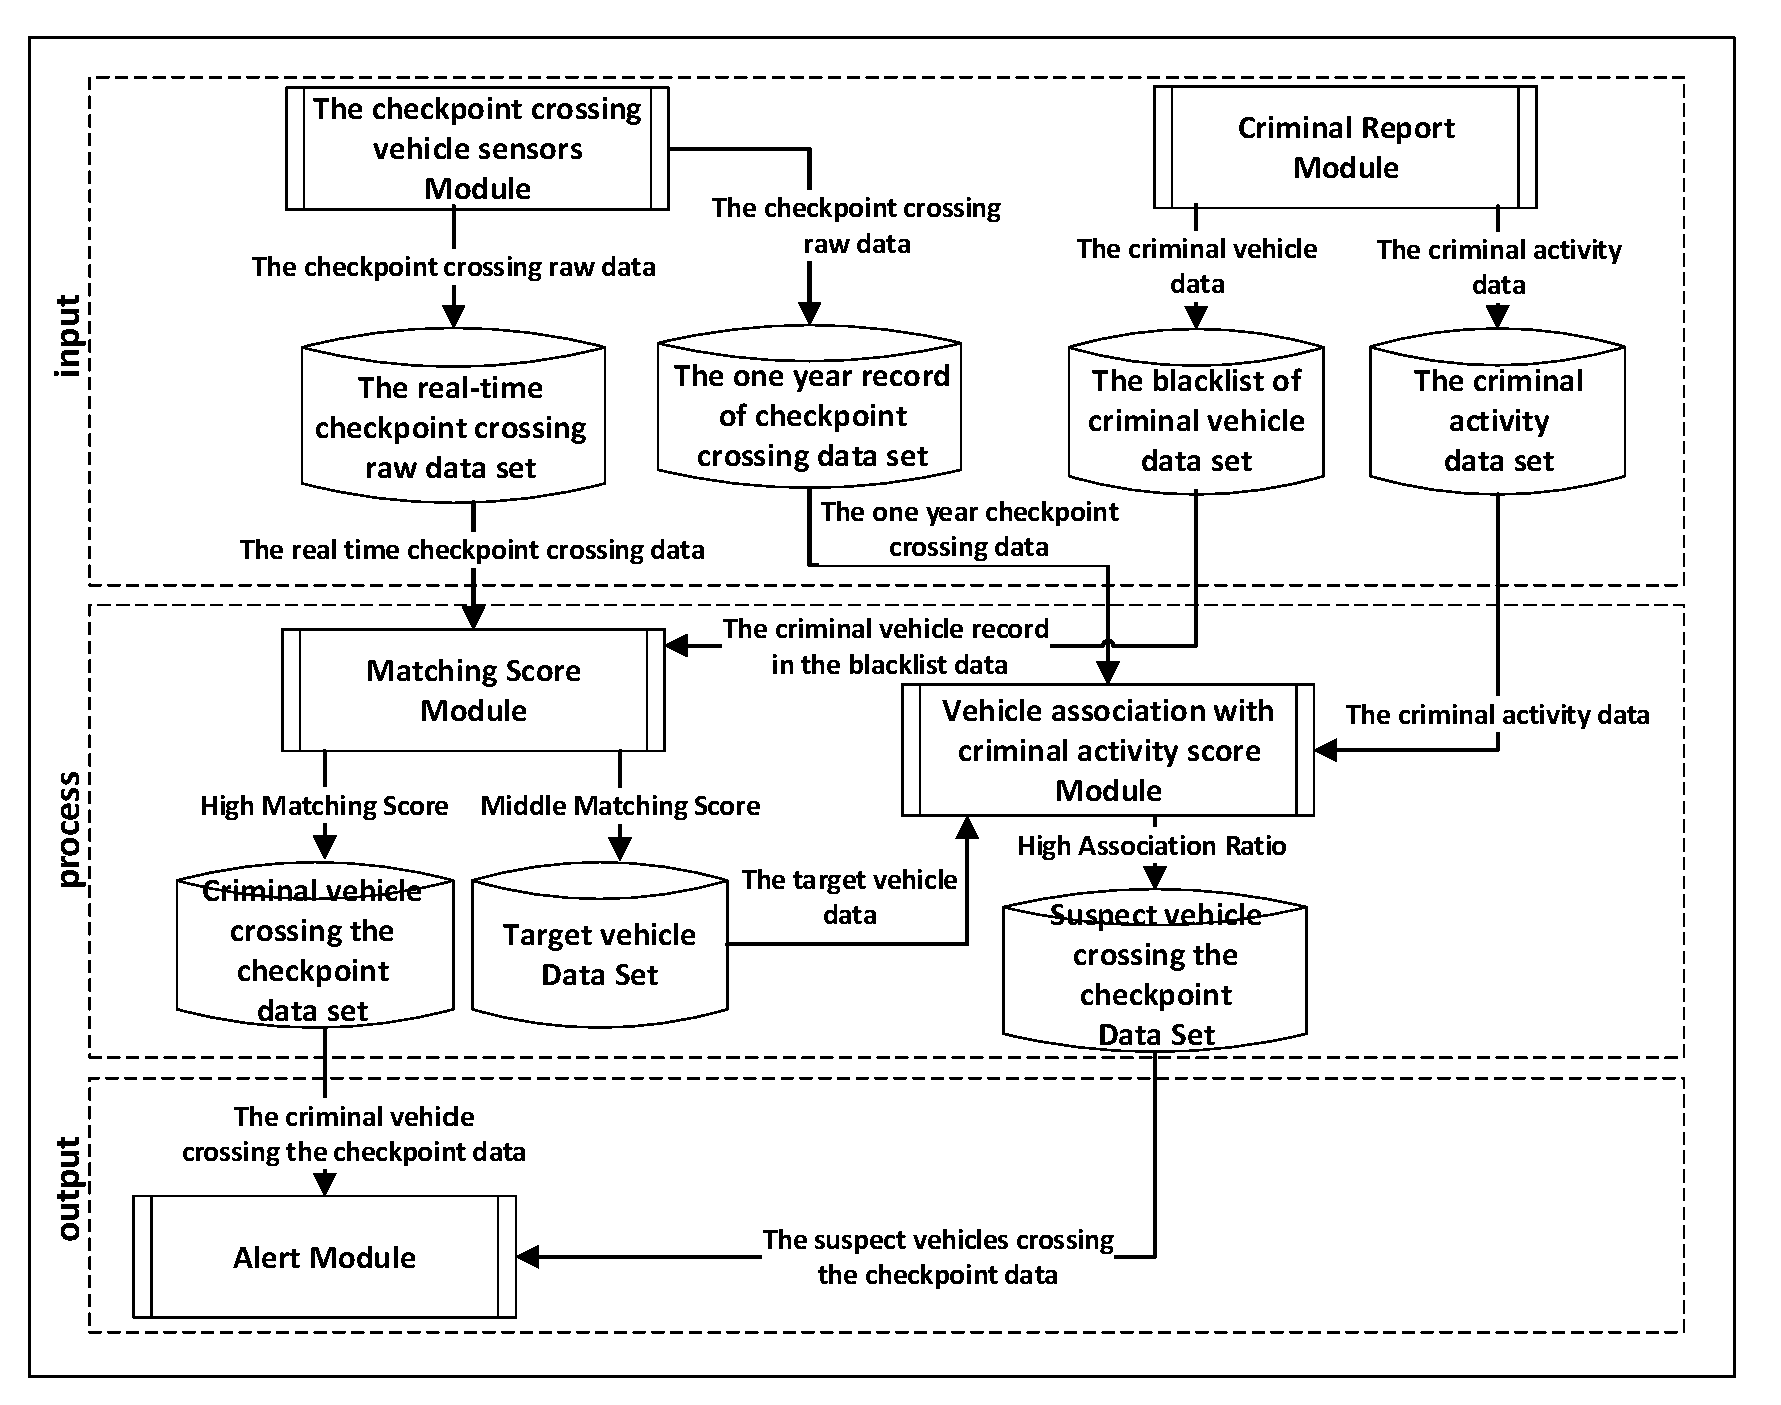
\includegraphics[width=1\textwidth]{images/myfigure.pdf}
\caption{Research design and process diagram.}
\label{fig:diagram}
\end{figure*}

Fig. \ref{fig:diagram} shows the research design and the evolution process of criminal or suspect vehicle detection at the checkpoint. This diagram is divided into three sections: 
1) Input section consists of the real time checkpoint crossing data set in three months, the one year records of checkpoint crossing data set, the blacklist of criminal vehicle data set, and criminal activity data set. 
2) Processing section consists of matching score module to detect the criminal vehicles that crossing the checkpoint and vehicle association with criminal activity score module to detect the suspect vehicles that crossing the checkpoint. In this research, we focus on the processing section shown in Fig.\ref{fig:diagram} which is explained in the following sub-sections. 
3) Output section serves as the alert of the criminal vehicle or suspect vehicle if the system detects the criminal vehicles or suspect vehicles that crossing the checkpoint. 

\subsubsection{Matching Score Module}
%
\begin{figure}
\vspace{1.8mm}
\centering
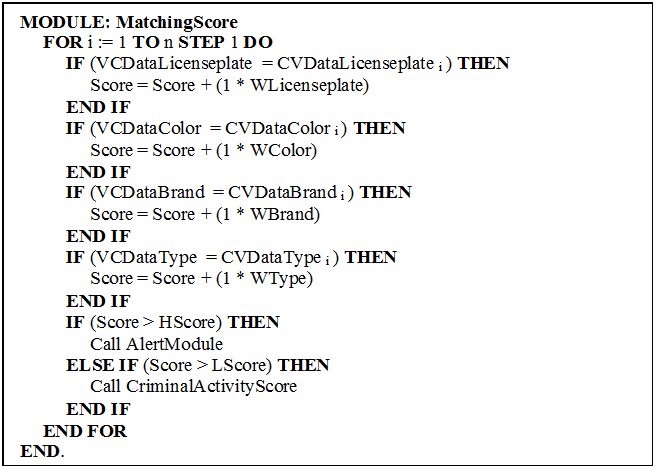
\includegraphics[width=1\textwidth]{images/MatchingAlgorithm.jpg}
\caption{Matching score module algorithm.}
\label{fig:matchingAlgo}
\end{figure}
%
Matching Score Module is criminal vehicle detection process. 
First, we define attributes for classification and assign weight to each of the attributes. 
Higher weight is assigned to higher significant attributes.
In this research, we select the license plate, vehicle color, vehicle brand, and vehicle type to be used in the classification and we assign higher weight to license plate than vehicle color, vehicle brand, and vehicle type. 
The system compares the real time checkpoint crossing records in three months and criminal vehicle records in the blacklist by using following attributes: license plate, vehicle color, vehicle brand, and vehicle type. 
Subsequently, it computes the sum of all of the weighted attribute. 
The weighted sum is a single number to compare with the threshold.  
If weighted sum is greater than the high score threshold, referred to as High Matching Score, vehicle crossing the checkpoint will be considered as criminal vehicle and will be processed in the Alert Module. 
If weighted sum is less than the high score threshold and also greater than the low score threshold, referred to as Middle Matching Score, vehicle crossing the checkpoint will be considered as target vehicle and will be processed in the Vehicle Association with Criminal Activity Score Module. 
%put these in Notation table
\begin{table}
\caption{Variable Description for Matching Score Module}
\label{table_variableMatching}
\begin{center}
\renewcommand{\arraystretch}{1.4}
\setlength\tabcolsep{3pt}
\begin{tabular}{ll}
\hline\noalign{\smallskip}
$Variables$ & $Description$\\
\noalign{\smallskip}
\hline
\noalign{\smallskip}
 VCDataLicenseplate & The license plate of vehicle that crossing the checkpoint. \\
VCDataColor & The color of vehicle that crossing the checkpoint.\\
VCDataBrand & The brand of vehicle that crossing the checkpoint.\\
VCDataType & The type of vehicle that crossing the checkpoint.\\
CVDataLicenseplate & The license plate of the criminal vehicle.\\
CVDataColor & The color of the criminal vehicle.\\
CVDataBrand & The brand of the criminal vehicle.\\
CVDataType & The type of the criminal vehicle.\\
WLicenseplate & The weight of license plate.\\
WColor & The weight of vehicle color.\\
WBrand & The weight of vehicle brand.\\
WType & The weight of vehicle type.\\
Score & The sum of all of the weighted attribute.\\
HScore & The high score threshold.\\
LScore & The low score threshold.\\
\hline
\end{tabular}
\end{center}
\end{table}

High Matching Score is calculated by the following attribute-matching condition: at least license plate matches with the blacklist.
Middle Matching Score is calculated by the following attribute-matching condition: vehicle color and vehicle brand and vehicle type match with the blacklist. 
Algorithm of Matching Score Module is shown in Fig. \ref{fig:matchingAlgo}. Table \ref{table_variableMatching} summarizes the notation for Matching Score Module.

\subsubsection{Vehicle Association with Criminal Activity Score Module}
This module is a suspect vehicle detection process using association analysis concept to identify the vehicles that are potentially involved in criminal activities. 
We determine the number of all the one year checkpoint crossing lists of target vehicle by considering the matching of license plate, vehicle color, vehicle brand, and vehicle type. 
Consequently, we analyze the relationship between each of the criminal activity with all the one year checkpoint crossing records of target vehicle, and we further restricted the set to contain only checkpoint crossing records of target vehicle that already crossed the checkpoint near the location, date, and time of criminal activities. 
Such set can be indicated the number of involvement in criminal activities of target vehicle. 
Then we can calculated the association ratio by using in (1) by computing the fraction of number of involvement in criminal activities of target vehicle and number of the checkpoint crossing records of target vehicle to compare with the defined threshold.
\begin{eqnarray} 
\alpha \quad =\quad \frac { \nu  }{ \varsigma  }
\end{eqnarray}
where\mbox{ }\\
$\alpha$ = association ratio. \mbox{ }\\
$\nu$ = number of involvement in criminal activities of target vehicle.\mbox{ }\\
$\varsigma$ = total of the 1 year checkpoint crossing records of target vehicle.\\

If the vehicles with higher ratio than the threshold, they are considered potential suspect vehicles, and then the vehicle data will be processed in the Alert Module. 
Algorithm of Vehicle association with Criminal Activity Score Module is shown in Fig. \ref{fig:activityAlgo}. Table \ref{table_variableActivity} summarizes the notation for Vehicle Association with Criminal Activity Score Module.

\begin{figure}
%\vspace{1.8mm}
\centering
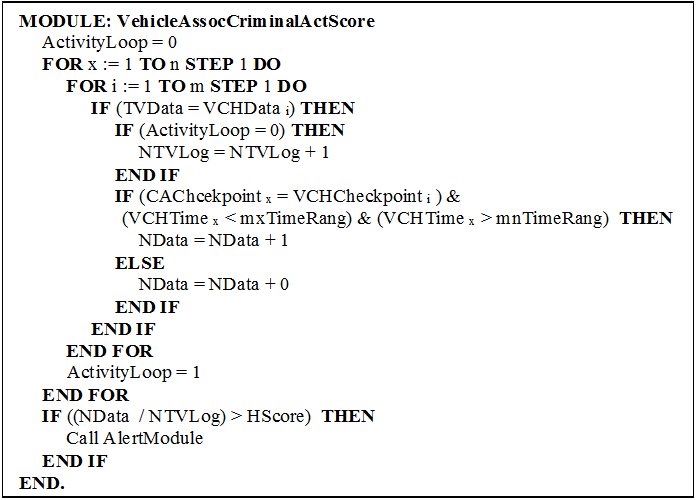
\includegraphics[width=1\textwidth]{images/activityAlgorithm2.jpg}
\caption{Vehicles association with criminal activity score module algorithm.}
\label{fig:activityAlgo}
\end{figure}

%put these in Notation table
\begin{table}
\caption{Variable Description for Vehicle Association with Criminal Activity Score Module}
\label{table_variableActivity}
\begin{center}
\renewcommand{\arraystretch}{1.4}
\setlength\tabcolsep{3pt}
\begin{tabular}{ll}
\hline\noalign{\smallskip}
$Variables$ & $Description$\\
\noalign{\smallskip}
\hline
\noalign{\smallskip}
ActivityLoop & The variable that used to check first iteration in x loop.\\
TVData & The target vehicle data includes license plate, 
vehicle color, \\ & vehicle brand, and vehicle type.\\
VCHData & The one year record of checkpoint crossing data set includes  \\ & license plate, vehicle color, vehicle brand, and vehicle type.\\
NTVLog & Total of one year checkpoint crossing records of target vehicle.\\
CAChcekpoint & The checkpoint near the location of the criminal activity.\\
VCHCheckpoint & The checkpoint that target vehicle has ever passed.\\
VCHTime & Date and time of the checkpoint crossing record.\\
mxTimeRang & Date and time of the criminal activity plus 1 hour.\\
mnTimeRang & Date and time of the criminal activity minus 1 hour.\\
NData & Number of involvement in criminal activities of target vehicle.\\
HScore & The defined threshold.\\
\hline
\end{tabular}
\end{center}
\end{table}

\section{Experimental Results}
To analyze system performance, there are four factors for analysis as follows:
1) True positive (TP) is the number of the criminal and suspect vehicles that are analyzed as the criminal and suspect vehicles.  
2) True negative (TN) is the number of the normal vehicles that are analyzed as the normal vehicles. 
3) False positive (FP) is the number of the normal vehicles that are analyzed as the criminal and suspect vehicles. 
4) False negative (FN) is the number of the criminal and suspect vehicles that are analyzed as the normal vehicles. 
Such factors can be calculated by using this formula:\\
$$ \text{TP Rate} =  \frac{\text{NofCSVDetectedAsCSV}}{\text{TofCSV}} $$\\
$$ \text{FN Rate} =  \frac{\text{NofCSVDetectedAsNV}}{\text{TofCSV}} $$\\
$$ \text{TN Rate} =  \frac{\text{NofNVDetectedAsNV}}{\text{TofNV}} $$\\ 
$$ \text{FP Rate} =  \frac{\text{NofNVDetectedAsCSV}}{\text{TofNV}} $$\\
$$ \text{Detection Accurate Rate} =  \frac{\text{TP Rate + TN Rate}}{\text{2}} $$

%put this in Notation
\begin{table}
\caption{Variable Description for The System Performance Analysis}
\label{table_variableSysPerf}
\begin{center}
\renewcommand{\arraystretch}{1.4}
\setlength\tabcolsep{3pt}
\begin{tabular}{ll}
\hline\noalign{\smallskip}
$Variables$ & $Description$\\
\noalign{\smallskip}
\hline
\noalign{\smallskip}
NofCSVDetectedAsCSV & The number of the criminal and suspect vehicles that \\ & are detected as the criminal and suspect vehicle.\\
TofCSV & The total of all the criminal and suspect vehicles.\\
NofCSVDetectedAsNV & The number of the criminal and suspect vehicles that \\ & are detected as the normal vehicle.\\
NofNVDetectedAsNV & The number of the normal vehicles that are detected \\ & as the normal vehicle.\\
TofNV & The total of all the normal vehicles.\\
NofNVDetectedAsCSV & The number of the normal vehicles that are detected \\ & as the criminal and suspect vehicle.\\
\hline
\end{tabular}
\end{center}
\end{table}

\begin{table}
\caption{Summary of The Vehicles Detected in Three Months}
\label{table_vehiclesDetected}
\begin{center}
\renewcommand{\arraystretch}{1.4}
\setlength\tabcolsep{3pt}
\begin{tabular}{lrr}
\hline\noalign{\smallskip}
$Vehicle Detection$ & $Traditional Process$ & $Novel Process$\\
\noalign{\smallskip}
\hline
\noalign{\smallskip}
Criminal Vehicles & 106 & 106\\
Suspect Vehicles & 0 & 147\\
\hline
\end{tabular}
\end{center}
\end{table}

\begin{table}
\caption{The Results of The System Performance Analysis}
\label{table_results}
\begin{center}
\renewcommand{\arraystretch}{1.4}
\setlength\tabcolsep{3pt}
\begin{tabular}{lrr}
\hline\noalign{\smallskip}
$Analysis Rate$ & $Traditional Process$ & $Novel Process$\\
\noalign{\smallskip}
\hline
\noalign{\smallskip}
TP Rate & 20.66\% & 49.32\%\\
FN Rate & 79.34\% & 50.68\%\\
TN Rate & 100\% & 98.87\%\\
FP Rate & 0\% & 1.13\%\\
Detection Accurate Rate & 60.33\% & 74.09\%\\
\hline
\end{tabular}
\end{center}
\end{table}

\begin{figure}
%\vspace{1.8mm}
\centering
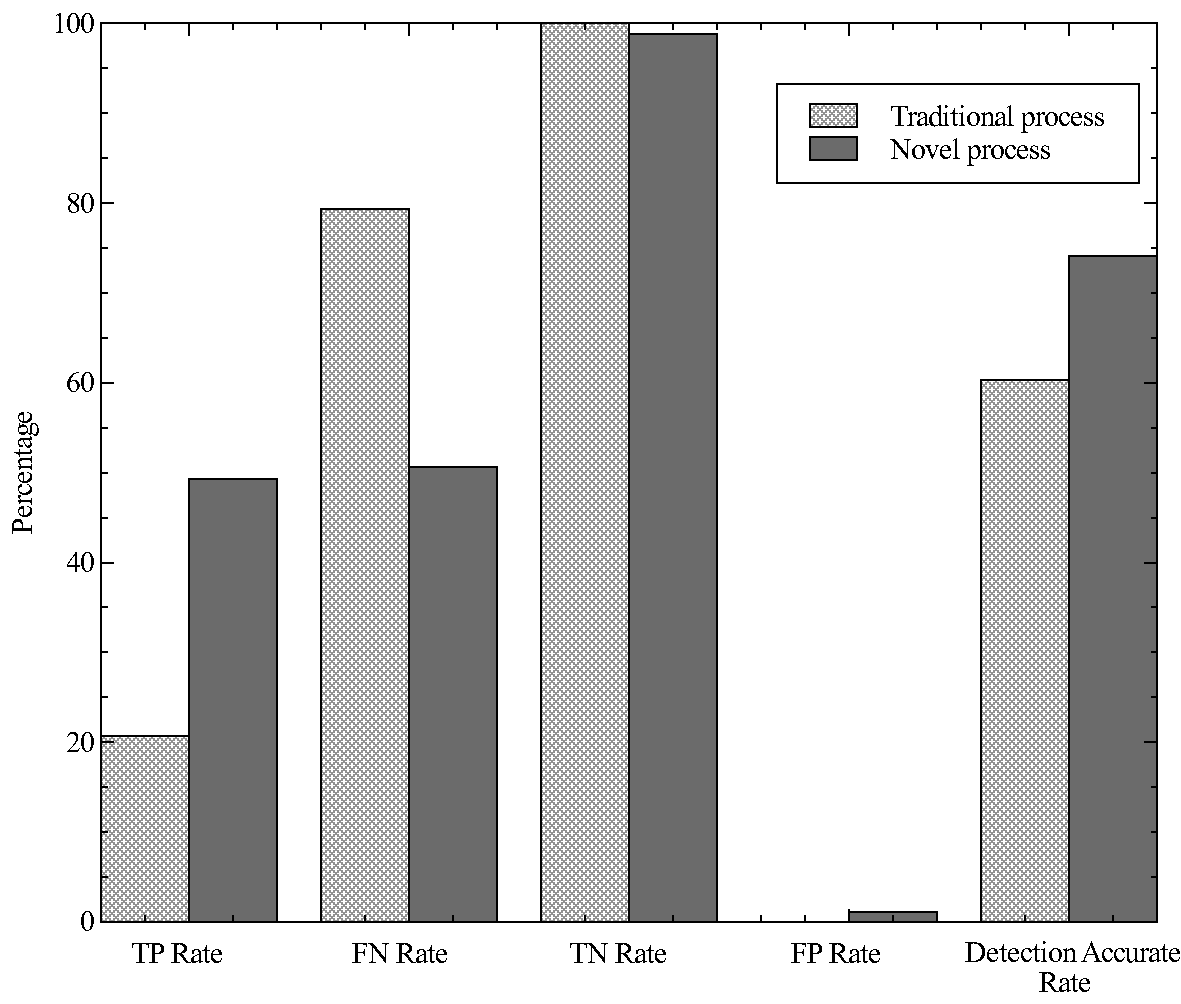
\includegraphics[width=0.9\textwidth]{images/results.pdf}
\caption{The results of the system performance analysis.}
\label{fig:graphresults}
\end{figure}

Table \ref{table_variableSysPerf} summarizes the notation for The System Performance Analysis.
The results obtained from the vehicle detection tests in three months is shown in Table \ref{table_vehiclesDetected}.
As a results, this novel process can detect 147 suspect vehicles more than the traditional process or equal to 138.68\% higher.
Fig. \ref{fig:graphresults} and Table \ref{table_results} show the results of the system performance analysis of the novel process that have the criminal or suspect vehicle detection rate is equal to 49.32\% and detection accurate rate is equal to 74.09\% which is an acceptable accurate rate. These results show that this technique can improve the detection capability of the suspect vehicle detection process.

\section{Discussion}
The novel process still gain higher FP rate than the traditional process because using only color, brand and type of vehicles matching the blacklist can not separate the normal vehicles out of the target vehicles. However, we intend to improve the normal vehicle separation process by using the target vehicle data from Matching Score Module matching the vehicle database of Department of Land Transport (DLT), Thailand. If the target vehicle data do not match the DLT database, it is considered as the illegal vehicles and processed in the Vehicle Association with Criminal Activity Score Module. In addition, the use of the DLT database can improve the FN rate.

\section{Conclusion and Future Directions}
This research proposes the use of vehicle reputation in couple with association analysis concept to improve the detection capability of suspect vehicle detection system.
The testing results from the previous section shows that the blacklist of criminal vehicles and criminal activity records obtained from criminal report database of DTI can be used to enhance the detection capability of suspect vehicle detection system and can address the limitations existing in the traditional process. 
In the future work, we plan to test this algorithm with the real scenario to compare with the formula in this research. 
In addition, we intend to explore the behavior of criminal vehicles crossing the checkpoint. This will allow us to analyze the crossing the checkpoint patterns of criminal vehicles and improve the suspect vehicle detection. Additionally, we intend to extend the suspect vehicle detection by using the vehicle crossing the checkpoint matching the vehicle database of DLT. This can be used to detect the illegal vehicles for reducing error of the normal vehicles detected as the suspect vehicles.


%\bibauthoryear
%
% ---- Bibliography ----
%
\begin{thebibliography}{15}
%

\bibitem{ZezhiChen}
Z. Chen, N. Pears, M. Freeman, and J. Austin: A gaussian mixturemodel and support vector machine approach to vehicle type and colour classification, Intelligent Transport Systems, IET, vol. 8, no. 2, pp. 135-144, March 2014.

\bibitem{Friedman}
N. Friedman and S. Russell: Image segmentation in video sequences: A probabilistic approach, in Proceedings of the Thirteenth Conference on Uncertainty in Artificial Intelligence, ser. UAI'97. San Francisco, CA, USA: Morgan Kaufmann Publishers Inc., 1997, pp. 175-181. [Online]. Available: http://dl.acm.org/citation.cfm?id=2074226.2074247

\bibitem{Stauffer}
C. Stauffer and W. Grimson: Learning patterns of activity using real-time tracking, Pattern Analysis and Machine Intelligence, IEEE Transactions on, vol. 22, no. 8, pp. 747-757, Aug 2000.

\bibitem{Hsieh}
J.-W. Hsieh, L.-C. Chen, and D.-Y. Chen: Symmetrical surf and its applications to vehicle detection and vehicle make and model recognition, Intelligent Transportation Systems, IEEE Transactions on,
vol. 15, no. 1, pp. 6-20, Feb 2014.

\bibitem{kaza:suspectVehicle}
S. Kaza and H. Chen: Suspect vehicle identification for border safety, in Intelligence and Security Informatics, ser. Studies in Computational Intelligence, H. Chen and C. Yang, Eds. Springer Berlin Heidelberg, 2008, vol. 135, pp. 305-318. [Online]. Available: http://dx.doi.org/10.1007/978-3-540-69209-6\_16

\bibitem{kaza} S. Kaza, T.Wang, H. Gowda, and H. Chen: Target vehicle identification for border safety using mutual information, in Intelligent Transportation Systems, 2005. Proceedings. 2005 IEEE, Sept 2005, pp. 1141-1146.

\bibitem{Umedu}
T. Umedu, K. Isu, T. Higashinoz, and C.-K. Toh: An intervehicular-communication protocol for distributed detection of dangerous vehicles, Vehicular Technology, IEEE Transactions on, vol. 59, no. 2, pp. 627-637, Feb 2010.

\bibitem{kaza:TopologicalAnalysis}
S. Kaza, J. Xu, B. Marshall, and H. Chen: Topological analysis of criminal activity networks: Enhancing transportation security, Intelligent Transportation Systems, IEEE Transactions on, vol. 10, no. 1, pp. 83-91, March 2009.

\bibitem{Thiel}
G. Thiel: Automatic cctv surveillance-towards the virtual guard, Aerospace and Electronic Systems Magazine, IEEE, vol. 15, no. 7, pp. 3-9, Jul 2000.

\bibitem{QinLi}
Q. Li, A. Malip, K. Martin, S.-L. Ng, and J. Zhang: A reputation-based announcement scheme for vanets, Vehicular Technology, IEEE Transactions on, vol. 61, no. 9, pp. 4095-4108, Nov 2012.

\bibitem{Dhurandher}
S. Dhurandher, M. Obaidat, A. Jaiswal, A. Tiwari, and A. Tyagi: Vehicular security through reputation and plausibility checks, Systems Journal, IEEE, vol. 8, no. 2, pp. 384-394, June 2014.

\bibitem{Ayday}
E. Ayday and F. Fekri: An iterative algorithm for trust management and adversary detection for delay-tolerant networks, Mobile Computing, IEEE Transactions on, vol. 11, no. 9, pp. 1514-1531, Sept 2012.

\bibitem{Xie}
M. Xie and H. Wang: A collaboration-based autonomous reputation system for email services, in INFOCOM, 2010 Proceedings IEEE, March 2010, pp. 1-9.
%\bibitem{DBLP:taylor} Bradley Taylor: Sender reputation in a large webmail service, in CEAS, 2006.

%\bibitem{Wang:ARTSense}
%X. Wang, W. Cheng, P. Mohapatra, and T. Abdelzaher: Artsense: Anonymous reputation and trust in participatory sensing, in INFOCOM, 2013 Proceedings IEEE, April 2013, pp. 2517-2525.
%\bibitem{lazzari} Lazzari, L. and Mari, M. and Poggi, A.: A collaborative and multi-agent system for e-mail filtering and classification, in Collaborative Computing: Networking, Applications and Worksharing, 2005 International Conference on, 2005, pp. 8 pp.-

\bibitem{Chirita:Mailrank} 
P.-A. Chirita, J. Diederich, and W. Nejdl: Mailrank: Using ranking for spam detection, in Proceedings of the 14th ACM International Conference on Information and Knowledge Management, ser. CIKM '05. New York, NY, USA: ACM, 2005, pp. 373-380. [Online]. Available: http://doi.acm.org/10.1145/1099554.1099671

\bibitem{West:Spam} 
A. G. West, A. J. Aviv, J. Chang, and I. Lee: Spam mitigation using spatio-temporal reputations from blacklist history, in Proceedings of the 26th Annual Computer Security Applications Conference, ser. ACSAC '10. New York, NY, USA: ACM, 2010, pp. 161-170. [Online]. Available: http://doi.acm.org/10.1145/1920261.1920287

\bibitem{Zhang:Ipgrouprep}
H. Zhang, H. Duan, W. Liu, and J. Wu: Ipgrouprep: A novel reputation based system for anti-spam, in Ubiquitous, Autonomic and Trusted Computing, 2009. UIC-ATC '09. Symposia and Workshops on, July 2009, pp. 513-518.

\bibitem{altman} 
A. Altman and M. Tennenholtz: Ranking systems: The pagerank axioms, in Proceedings of the 6th ACM Conference on Electronic Commerce, ser. EC '05. New York, NY, USA: ACM, 2005, pp. 1-8.
[Online]. Available: http://doi.acm.org/10.1145/1064009.1064010

%\bibitem{ding} Qing Ding and Xi Li and Ming Jiang and Xuehai Zhou: Reputation management in vehicular ad hoc networks, in Multimedia Technology (ICMT), 2010 International Conference on, Oct 2010, pp. 1-5.

%\bibitem{park} Soyoung Park and Aslam, B. and Zou, C.: Long-term reputation system for vehicular networking based on vehicle's daily commute routine, in Consumer Communications and Networking Conference (CCNC), 2011 IEEE, Jan 2011, pp. 436-441.

\bibitem{page} Page, L. and Brin, S. and Motwani, R. and Winograd, T.: The pagerank citation ranking: Bringing order to the web, in Proceedings of the 7th International World Wide Web Conference, Brisbane, Australia, 1998, pp. 161-172. [Online]. Available: http://citeseer.nj.nec.com/page98pagerank.html

\bibitem{WangLin}
Y. Wang and K.-J. Lin: Reputation-oriented trustworthy computing in e-commerce environments, Internet Computing, IEEE, vol. 12, no. 4, pp. 55-59, July 2008.
%\bibitem{resnick} Resnick, Paul and Zeckhauser, Richard: Trust among strangers in Internet transactions: Empirical analysis of eBay\'s reputation system, in The Economics of the Internet and E-Commerce, ser. Advances in Applied Microeconomics, M. R. Baye, Ed. Elsevier Science, 2002, vol. 11, pp. 127-157. [Online]. Available: http://www.si.umich.edu/ presnick/papers/ebayNBER/index.html

\bibitem{chruch} Church, Kenneth Ward and Hanks, Patrick: Word association norms, mutual information, and lexicography, Comput. Linguist., vol. 16, no. 1, pp. 22-29, Mar. 1990. [Online]. Available: http://dl.acm.org/citation.cfm?id=89086.89095

\bibitem{romashchenko} Romashchenko, A.: Extracting the mutual information for a triple of binary strings, in Computational Complexity, 2003. Proceedings. 18th IEEE Annual Conference on, July 2003, pp. 221-229.

\bibitem{Exarchos}
T. Exarchos, C. Papaloukas, D. Fotiadis, and L. Michalis: An association rule mining-based methodology for automated detection of ischemic ecg beats, Biomedical Engineering, IEEE Transactions on, vol. 53, no. 8, pp. 1531-1540, Aug 2006.
%\bibitem{li} Li Xiang-wei and Zhao Shuang-ping: A novel web authoritative page mining algorithm based on association analysis, in Knowledge Acquisition and Modeling (KAM), 2011 Fourth International Symposium on, Oct 2011, pp. 136-138.

\bibitem{zhuang} Ziyun Zhuang and Bo Zhang: Application of association analysis in digital content industry, in Computational Intelligence and Design (ISCID), 2012 Fifth International Symposium on, vol. 1, Oct 2012, pp. 18-21.

\bibitem{miao} Miao, Gengxin and Guan, Ziyu and Moser, Louise E. and Yan, Xifeng and Tao, Shu and Anerousis, Nikos and Sun, Jimeng: Latent association analysis of document pairs, in Proceedings of the 18th ACM SIGKDD International Conference on Knowledge Discovery and Data Mining, ser. KDD '12. New York, NY, USA: ACM, 2012, pp. 1415-1423. [Online]. Available: http://doi.acm.org/10.1145/2339530.2339752

\end{thebibliography}
%
\end{document}
